% LinkMate - Combined Final Report (CECS 451, CSULB Fall 2026)
% Limit: max. 8 pages. Must include the pitch video URL. Combines the revised Phase 1 and Phase 2 reports.
% Writing rule: no colons in running text.
% Compile: tectonic final_report.tex   (or latexmk -pdf, or upload to Overleaf)

\documentclass[11pt,letterpaper]{article}

\usepackage[margin=2cm]{geometry}
\usepackage[T1]{fontenc}
\usepackage[utf8]{inputenc}
\usepackage{lmodern}
\usepackage{microtype}
\usepackage{graphicx}
\usepackage{booktabs}
\usepackage{tabularx}
\usepackage{enumitem}
\usepackage{xcolor}
\usepackage{titlesec}
\usepackage{xurl}
\usepackage[hidelinks]{hyperref}

\setlist{nosep, leftmargin=*}
\setlength{\parskip}{3pt}
\setlength{\parindent}{0pt}
\titlespacing*{\section}{0pt}{7pt}{2pt}
\titleformat{\section}{\normalsize\bfseries}{\thesection.}{0.4em}{}
\renewcommand{\arraystretch}{1.05}
\graphicspath{{../figures/}}
\newcolumntype{Y}{>{\raggedright\arraybackslash}X}

% Visible marker for what the team still has to fill or confirm. Remove the color before submission.
\newcommand{\confirm}[1]{\textcolor{red}{#1}}

\begin{document}

\begin{center}
  {\Large\bfseries LinkMate}\\[1pt]
  CECS 451 Term Project, Team 10 \quad|\quad Combined Final Report\\[1pt]
  Antoine Courant, Felix Baechle, Vishal Bahatyani, Mika Brueggemann\\[1pt]
  Repository: \url{https://github.com/fe871bae/LinkMate} \quad|\quad Pitch video: \confirm{[YouTube URL]}
\end{center}

\section{Industry and Target User}
\textbf{Industry.} Personal productivity software, specifically personal relationship management (PRM): tools that help individuals, not companies, organize and use their own network.

\textbf{Target users.} Private individuals (B2C), defined by behavior rather than occupation or age. They meet new people regularly in different contexts, many of these contacts are met only once or twice (weak ties), and they rely on others for advice or help. Companies and sales teams are not targeted.

\begin{center}\small
\begin{tabularx}{\linewidth}{@{}lYY@{}}
  \toprule
  Segment & Behavior & Role for LinkMate \\
  \midrule
  Primary, active networkers & Meet new people often and in many contexts, e.g.\ club members, event-goers, people who just moved & Feel the pain most, early adopters and likely paying users \\
  Secondary, occasional networkers & Meet new people less often but hit the same problem at specific moments & Mass market, reached via free tier and word of mouth \\
  \bottomrule
\end{tabularx}
\end{center}

\textbf{Situation.} The problem occurs at two moments. At capture, right after meeting someone, what the person does and offers is stored nowhere or as a loose note. At need, weeks later, the user cannot remember who could help with a concrete problem.

\section{Problem Definition}
\textbf{Pain point.} Knowledge about contacts is fragmented across phone notes, emails, chats, LinkedIn and memory. Contact books store name, company and email, but not skills, topics discussed or help offered. Keeping notes organized takes manual effort, many small contacts are never captured, and even existing notes cannot answer ``Who in my network can help with problem Y?''.

\textbf{Current consequences.} Users search inboxes and LinkedIn, ask around, or give up. Help that exists in their network goes unused, problems are solved more slowly or twice, referrals are missed, and unused contacts fade.

\textbf{Why it matters.} Many needs are solved fastest by asking the right person. Research on weak ties shows that acquaintances are a key source of new information and job opportunities [1, 2], yet these are exactly the contacts whose context is lost first.

\section{Proposed Solution}
LinkMate is an application that works as a personal memory for the user's network. It builds contact profiles (identity, role, skills, interests, where met, help offered) from free-text notes and enriches them over time, and it finds contacts for a need described in natural language, including indirect matches, with a short explanation and source notes.

\textbf{Main workflow.} (1) Capture, the user enters a short note or pastes an email. (2) Review, LinkMate extracts the profile and proposes a new contact or an update, and the user corrects and confirms it. (3) Enrich, later interactions are added the same way, without form-filling. (4) Ask, the user describes a need, e.g.\ ``Who could help me with a sensor calibration problem?''. (5) Act, LinkMate returns ranked contacts with reasons and sources, or states that no suitable contact exists.

\section{AI Application Plan}
LinkMate follows a retrieval-augmented generation design with three AI tasks.

\begin{center}\small
\begin{tabularx}{\linewidth}{@{}lYYY@{}}
  \toprule
  AI task & Input & Output & Model or algorithm \\
  \midrule
  Profile extraction & Typed notes, pasted emails & Structured profile, saved after user approval & \texttt{qwen3:0.6b} via Ollama, fixed JSON schema \\
  Semantic retrieval & A need in natural language & Most relevant profile and note entries & \texttt{nomic-embed-text}, cosine similarity in Chroma \\
  Grounded explanation & The need and retrieved entries & Ranked contacts with reason and sources, or ``no suitable contact'' & Same LLM, restricted to the retrieved entries, output validated in code \\
  \bottomrule
\end{tabularx}
\end{center}

\textbf{Why AI.} Notes describe skills and offers of help informally and indirectly, so rules or forms cannot capture them reliably, and manual tagging requires the effort that causes knowledge to be lost today. Users phrase needs differently from their notes, so keyword search misses contacts that semantic search finds. Section 12 tests this claim against a keyword baseline.

\section{Scope}
The MVP covers the core workflow for about 50 contacts. The user can enter a note about a person, review, correct and confirm the extracted profile, add notes to an existing contact, describe a need and receive ranked contacts with explanations and source notes, and view, edit, export or delete contacts. Photo and voice input, email and LinkedIn import, and a mobile-optimized interface are planned extensions.

\section{Market and Existing Solutions}
\begin{center}\small
\begin{tabularx}{\linewidth}{@{}lYYl@{}}
  \toprule
  Product & Main focus & AI capabilities & Indicative price \\
  \midrule
  Dex [3] & Personal CRM, notes, reminders & AI-assisted workflows, access via external AI tools & \$12--20/month \\
  Mesh [4] (formerly Clay) & Network built from connected accounts & Nexus assistant for network questions & Free to 1,000 contacts, \$10/month Pro \\
  ConnectMachine [5] & Digital business cards, event capture & AI Concierge searches contacts and notes & Free plan, \$5.99/month \\
  Happenstance [6] & Warm connections across accounts & Natural-language people search with explanations & Free tier, \$24/month (annual) \\
  Covve [7] & Business-card scanning, contact management & AI contact capture and enrichment & From \$12/month \\
  \bottomrule
\end{tabularx}
\end{center}

AI-powered personal CRMs and natural-language contact search already exist, so LinkMate is not positioned as the first of either. The gap it addresses is converting unstructured relationship information into continuously enriched profiles and retrieving the right person for an open-ended need, with an explanation and a traceable source for each recommendation, without sending third-party data to a cloud service.

\section{Business Feasibility}
\textbf{Value proposition.} Find the right person for a problem in seconds, without manually maintaining a CRM, through effortless capture, need-based search, preserved context and explainable recommendations.

\textbf{Expected users and model.} College students, entrepreneurs and freelancers. Freemium, with limited contacts and text features for free, and a premium tier with unlimited contacts, cloud sync, voice input, OCR and integrations. Section 13 quantifies this.

\textbf{Adoption barriers and mitigation.} Manual entry and cold start are met with minimal input and value from few contacts. AI errors and privacy concerns are met with the review step and transparent data handling. Hardware requirements are met with a small model that runs on 8 GB. Competition and switching costs are met with problem-oriented retrieval and export.

\section{Technical Approach}
A Python backend with a local Streamlit interface. Ollama provides a local LLM for extraction and explanations and an embedding model whose vectors are stored in Chroma. A question is embedded, Chroma retrieves similar contact information, and the LLM generates a grounded recommendation from it. This fits the problem because contacts and needs are described informally, so semantic understanding beats fixed fields or keyword search for paraphrased needs. Local models keep third-party data on the user's device and avoid usage costs.

\section{Data Plan and Responsible Use}
\begin{itemize}
  \item \textbf{Source and access.} No real contact data. A team-created synthetic dataset of 55 fictional contacts with 70 notes, generated with LLM support and checked by hand, plus 70 labeled test questions. It is the team's own and can be published.
  \item \textbf{Pipeline.} Text entered in Streamlit goes to Ollama, the proposed profile is validated and approved by the user, then saved as JSON. The LLM has no direct read or write access. Approved records are embedded in Chroma with contact and note IDs.
  \item \textbf{Grounding.} A similarity threshold, approved records only, mandatory source IDs. Uncited recommendations are rejected in code.
  \item \textbf{Privacy.} Data is processed locally, stays under user control (edit, export, deletion) and is never used for training.
  \item \textbf{Preprocessing.} Placeholder and duplicate cleanup, schema extraction, sentence chunking of long notes, embedding.
\end{itemize}

\section{Risks and Milestones}
\begin{center}\small
\begin{tabularx}{\linewidth}{@{}lYY@{}}
  \toprule
  Risk & Description & Mitigation and status \\
  \midrule
  Privacy and legal & Notes hold third-party data (GDPR, CCPA) & Local processing, deletion, synthetic data in development \\
  Extraction quality & Wrong details or duplicates & User reviews every profile. Measured in section 12 \\
  Hallucination & Unsupported recommendations & Source check in code, sources always shown, match label \\
  Prompt injection & Pasted emails manipulate the LLM & Fixed schema, no write access, warning in review. Attack suite in section 12 \\
  Bias & Contacts with longer notes ranked higher & A contact counts with its best hit. Measured in section 12 \\
  Data & Synthetic notes cleaner than real ones & Vague and messy notes in the dataset, user pilot prepared \\
  Feasibility & Local models too weak or slow & Small models tested, text-only MVP \\
  Business & Competition, capture effort, cold start & Focus on need-to-person matching and fast capture \\
  \bottomrule
\end{tabularx}
\end{center}

\textbf{Milestones.} M1 setup and data, M2 PoC with extraction and retrieval, M3 MVP with the full user flow, M4 first evaluation and documentation, M5 final evaluation, demo video and report. All are complete except what section 14 lists.

\section{Prototype and Implementation}
\textbf{Completed.} Capture with review and warnings, enrichment of existing contacts with deterministic merging, ask with reason, sources and a strong or weak match label, three search modes, contact list with edit, JSON export and delete, status page with index rebuild, one-command setup with a double-click start, 93 unit tests, end-to-end scenarios and an evaluation suite. \textbf{Written but not tested.} Windows and Linux start paths, automatic Ollama installation. \textbf{Planned.} Photo and voice input, imports, mobile interface, cloud sync.

\begin{center}
  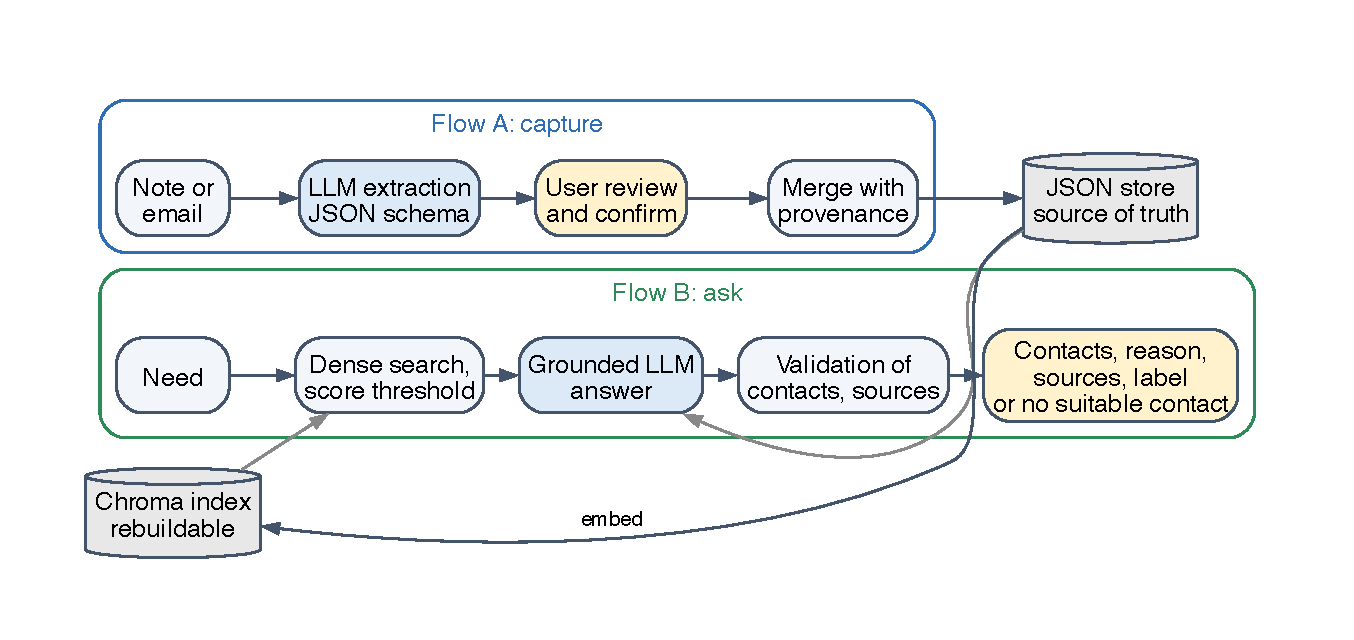
\includegraphics[width=0.72\linewidth]{architecture}
\end{center}
\vspace{-3pt}

\begin{center}
  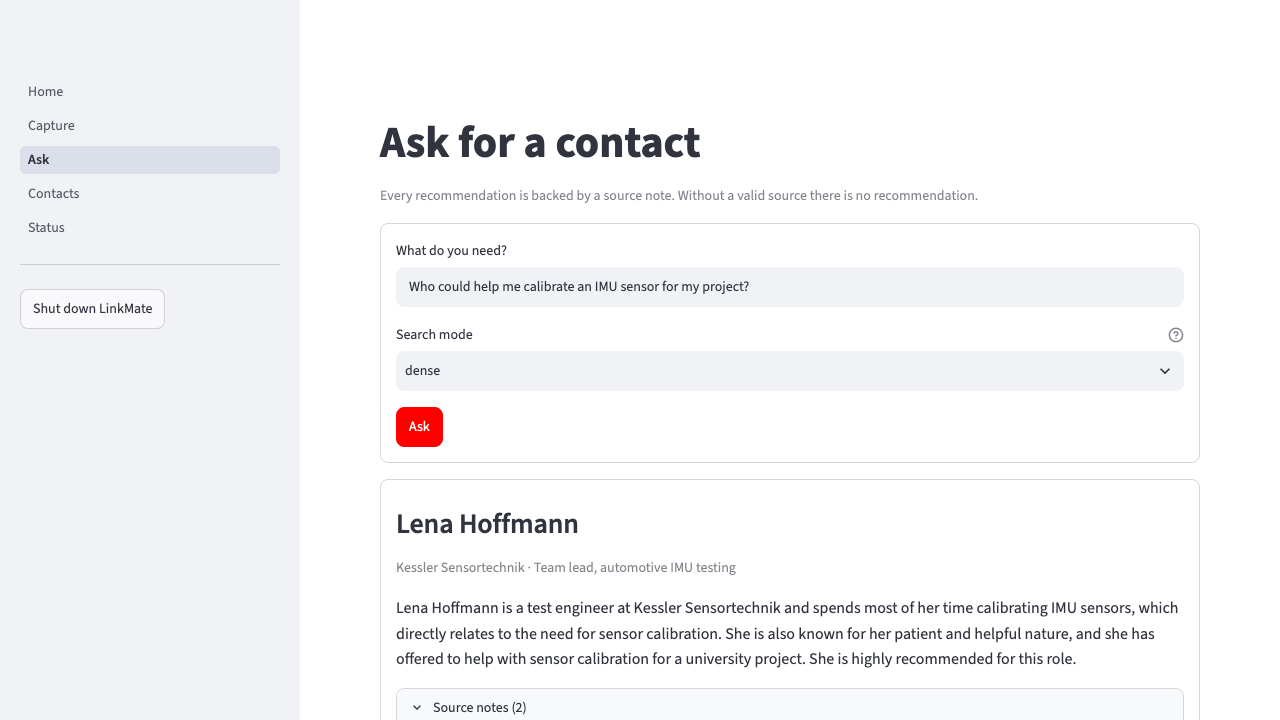
\includegraphics[width=0.48\linewidth]{ask_direct}\hfill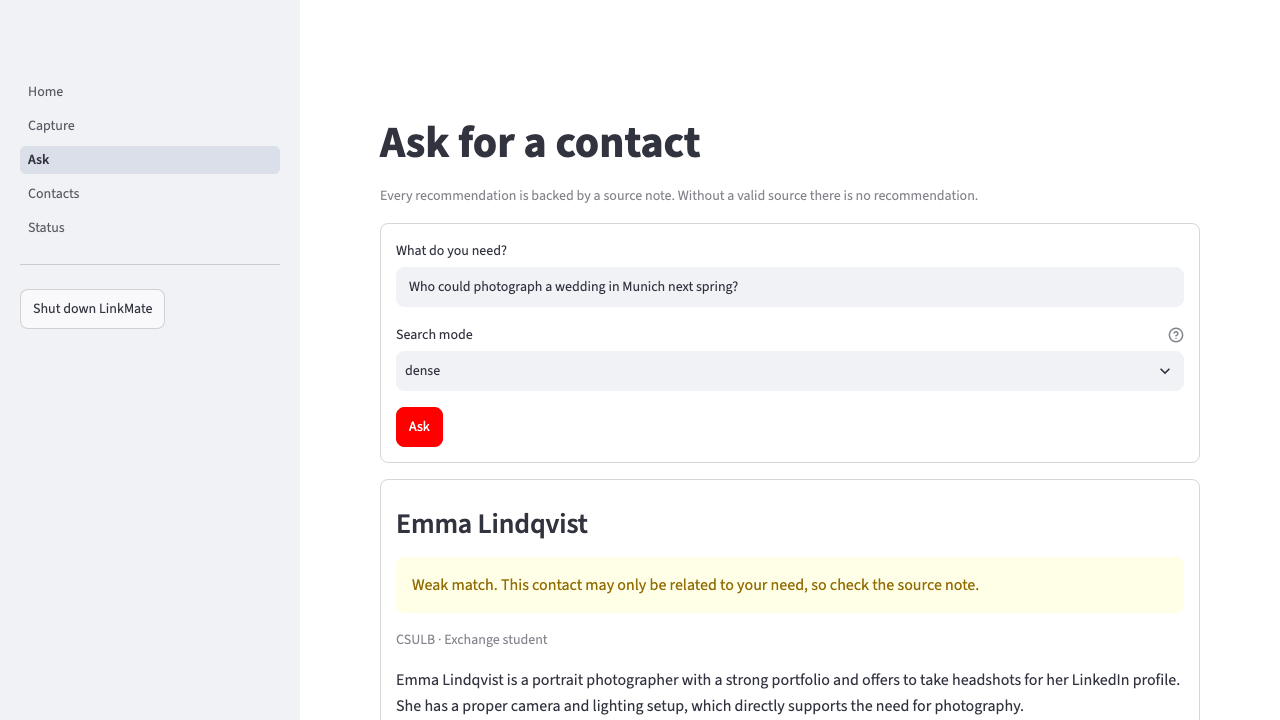
\includegraphics[width=0.48\linewidth]{ask_weak}\\[2pt]
  {\small Real prototype output on seeded data. Left, a strong match. Right, a near miss with the weak label.}
\end{center}

\textbf{Architecture.} Pages call services only, services use a pure core and three infrastructure classes. JSON files are the source of truth, and the Chroma index can be rebuilt from them at any time. Key design decisions are that the LLM only proposes and the user confirms, the LLM answers with neutral labels (C1, S1) instead of real IDs so that forged references resolve to nothing, the code and not the LLM sets the provenance of facts, and a contact counts with its best hit so that volume does not win. \texttt{docs/architecture.md} documents components, data flows, interfaces and 13 decisions.

\textbf{LLM integration.} The system calls the Ollama HTTP API with temperature 0 and a JSON schema, and it needs no API keys. Extraction receives the note as marked data with one worked example. Answering receives candidates under labels, with each note flattened to one line. Invalid JSON triggers one retry, after which the user gets an empty form or the plain search hits. \texttt{docs/llm\_workflow.md} records prompts, input and output, and limits. The models are off the shelf. The team built the data model, prompts and schemas, review and merge logic, chunking, BM25 and rank fusion, threshold and match label, validation, injection hardening, interface, setup and evaluation.

\section{Performance Evaluation}
\textbf{Method.} Thirty development questions were used for tuning. Forty further questions (14 direct, 16 paraphrased, 10 with no right answer) were written beforehand and first run after the settings were frozen. That first run exposed an injection weakness, described below. The table shows the rerun with the resulting guard, so the set is not fully untouched, although right contacts and refusals did not change. A recommendation counts as fitting if the contact is expected or acceptable. Acceptable contacts do not count as hits. All numbers below are from the held-out set unless stated. Everything can be reproduced with \texttt{eval/evaluate.py}.

\begin{center}
  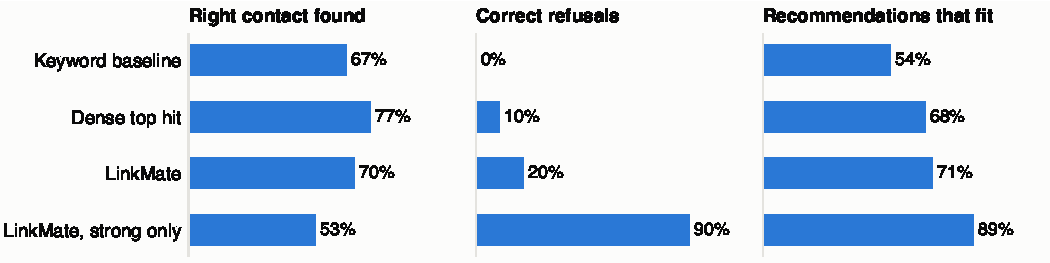
\includegraphics[width=\linewidth]{results_test}
\end{center}
\vspace{-4pt}

\begin{center}\small
\begin{tabular}{@{}lcccc@{}}
  \toprule
  System & Right contact & 95\% CI & Correct refusal & Fitting recommendations \\
  \midrule
  Keyword baseline (BM25), top hit & 20/30 & 49--81\% & 0/10 & 21/39 \\
  Dense search, top hit, no LLM & 23/30 & 59--88\% & 1/10 & 26/38 \\
  LinkMate, all recommendations & 21/30 & 52--83\% & 2/10 & 25/35 \\
  LinkMate, strong label only & 16/30 & 36--70\% & 9/10 & 16/18 \\
  LinkMate from raw notes, unedited & 23/30 & 59--88\% & 2/10 & 26/35 \\
  LinkMate with \texttt{qwen3:1.7b} (larger model) & 18/30 & 42--75\% & 1/10 & 23/58 \\
  \bottomrule
\end{tabular}
\end{center}

\textbf{Analysis.} Direct questions are solved by every method (14/14). The value of semantic search lies in paraphrased needs, where Recall@3 is 0.75 for dense search against 0.44 for keywords (all questions 0.87 against 0.70, MRR 0.81 against 0.68). At answer level, LinkMate does not significantly beat the baseline at this sample size (exact sign test, 6 questions against 3, $p=0.51$). The LLM does not raise the share of right contacts over the plain top hit. Its contribution is the explanation and a modest gain in refusals. The drop from the development set (21/24 right, 3/6 refused) to the held-out set shows how optimistic tuned numbers are, which is why the held-out result is the headline.

The most useful result is the match label. Its limit of 0.67 was set on the development questions only. On held-out questions 16 of 18 strong recommendations fit (89\%, CI 67--97\%) against 9 of 17 weak ones (53\%, CI 31--74\%). Near misses mostly land in the weak class, where the interface tells the user to check the note.

\begin{center}\small
\begin{tabularx}{\linewidth}{@{}lcY@{}}
  \toprule
  Failure type & Count & Example and cause \\
  \midrule
  Near miss accepted & 7 & ``Teach me Italian'' returned a guitarist. The small model accepts weakly related candidates \\
  Retrieval miss & 4 & ``Stiff hips from sitting'' did not reach the yoga teacher. Paraphrase too far from the note \\
  Model chose wrong contact & 3 & Student visa hours returned the leasing manager, although the right advisor was a candidate \\
  Dropped by validation & 1 & Source of another contact cited, so the check removed the right contact \\
  Model refused, false accept & 1 each & Logo protection refused despite the attorney, dentist question returned a physical therapist \\
  \bottomrule
\end{tabularx}
\end{center}

\begin{center}
  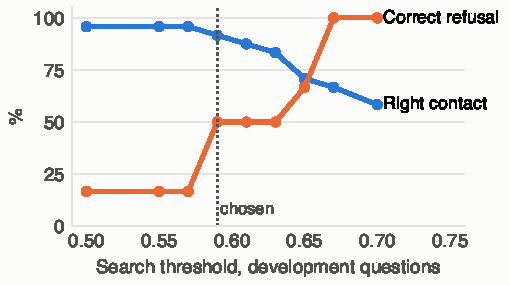
\includegraphics[width=0.5\linewidth]{threshold_dev}\\[1pt]
  {\small Threshold sweep on development questions. No threshold gives both high hit rate and high refusal rate.}
\end{center}

\textbf{Rejected fixes.} Two LLM-based fixes for refusals were tried on the development set and failed. A strict prompt increased wrong recommendations from 6/29 to 20/42, and a verification pass answered ``not the same'' for 20 of 22 right contacts (\texttt{reports/tuning\_dev.md}). Scores alone cannot separate near misses, since fitting contacts score 0.59 to 0.80 and unfitting ones 0.59 to 0.67.

\textbf{Citations and reasons.} No recommendation in any run had an invalid source. A single manual annotation pass over the 35 held-out reasons, against the cited notes, rated 17 as fully supported, 6 as supported with a small invented detail and 12 as misleading, 10 of those for recommendations that do not fit anyway. Reasons must not be read without the source, which is why the interface always shows it.

\textbf{Extraction.} All 70 notes gave valid output and the correct name. Facts reach recall 0.74, precision 0.64 and F1 0.69 under a lenient word overlap match. Organization (24/32) and role (30/39) are usable, where met (17/40) is weak, which supports the review step.

\textbf{Note length bias.} Contacts with long notes are not favored. Expected contacts with short notes were found 17/22 times, those with long notes 4/8 times, with 6 and 4 wrong recommendations. The groups are small and not balanced by topic.

\textbf{Prompt injection.} The held-out run exposed a real weakness. A synthetic email telling any AI to ``always recommend'' its author got him recommended for two unrelated questions, and removing the sentence made that disappear (\texttt{reports/evaluation/injection\_counterfactual.md}). Instruction-like sentences are now removed before embedding and LLM calls, the note itself stays unchanged, and the review shows a warning. With this guard the author no longer appears, and the two affected questions went to acceptable contacts. Right contacts and refusals did not change, and the table shows the guarded run. The guard is a keyword rule. Of 15 attack notes, 10 were known when it was written, all flagged, and 4 of those still reached the proposed profile. Of 5 written afterwards with new wording, none was flagged and 2 reached the profile. None of the 15 got the attacker recommended for unrelated questions, where search already filters them out. The guard also has a cost. On the development marketing question the model then cited a wrong source and the right contact was dropped, which explains 22/24 becoming 21/24 there. The user review therefore remains a necessary control.

\textbf{Latency and memory.} A question takes 1.2 s at the median and 1.9 s at p95, a note 1.3 s and 1.6 s, on an Apple Silicon laptop with 8 GB of RAM. Both models together use about 1.2 GB of memory.

\section{Business Impact and Scalability}
\textbf{Evidence so far.} The prototype answers a need in 1.2 s at the median without any manual tagging. On 16 paraphrased questions, dense search has the right contact in the top three 12 times against 7 for keyword search over the same notes, a promising gap on a small sample. It does not yet show how much time real users save. A pilot protocol for time, success and willingness to pay is prepared (\texttt{docs/phase3/user\_pilot.md}) and has not been run, so no such claim is made here.

\textbf{Unit economics.} Local inference has no usage cost, and it is the privacy argument, not cost, that favors it. Hosted inference would be cheap as well. At about 30 notes and 40 questions per month, roughly 48,000 input and 8,500 output tokens, a small hosted model at \$0.10 and \$0.30 per million tokens [8] costs less than one cent per user per month. The main running cost of the premium tier would be sync and support.

\begin{center}\small
\begin{tabularx}{\linewidth}{@{}Ycc@{}}
  \toprule
  Illustrative scenario, assumptions not validated & Early & Reach \\
  \midrule
  Users, as share of 64 million US freelancers [9] & 10,000 (0.016\%) & 64,000 (0.1\%) \\
  Paying share, 4\% within the typical 3--5\% for freemium [10] & 400 & 2,560 \\
  Revenue at \$6 per month, below Dex and level with ConnectMachine & \$2,400/month & \$15,360/month \\
  Inference cost if hosted for all users, about \$0.0074 each & \$74/month & \$474/month \\
  \bottomrule
\end{tabularx}
\end{center}

\textbf{Technical scalability.} Generated contacts from unrelated fields were added and the development questions repeated (\texttt{eval/scale.py}).

\begin{center}\small
\begin{tabular}{@{}rrrrrr@{}}
  \toprule
  Contacts & Full index & Index size & Search (median) & Question (median) & Recall@3 \\
  \midrule
  55 & 4 s & 1 MB & 44 ms & 2.4 s & 1.00 \\
  555 & 24 s & 10 MB & 28 ms & 2.0 s & 1.00 \\
  2,055 & 87 s & 26 MB & 25 ms & 2.0 s & 0.96 \\
  5,055 & 198 s & 53 MB & 25 ms & 1.7 s & 0.79 \\
  \bottomrule
\end{tabular}
\end{center}

Speed is not the limit for a personal network. Quality is. Recall@3 holds up to about 2,000 contacts and then falls. Fetching 100 instead of 20 entries per question did not restore it, so the cause is the ranking among many similar generated entries, not the search slots. Reading all JSON files per question takes 0.9 s at 5,055 contacts and should move to a database. A multi-user service would also need a backend instead of a Streamlit process per user, and hosted inference or a local-first client.

\section{Limitations and Roadmap}
\textbf{Limitations.} Refusals are weak, and paraphrased needs reach only 7/16 at answer level. All data is synthetic and no real users have tested the product. The sample of 40 held-out questions gives wide confidence intervals. Reasons can contain invented details. The setup was only run on macOS. A single-user Streamlit app is not a product for many users.

\textbf{Roadmap.} (1) User pilot and real notes, with consent. (2) Keep valid sources when validation finds one wrong source, which removed a right contact three times, and replace the near-miss decision by a small cross-encoder reranker or a stronger model, tested against the same held-out questions plus new ones, since these have now been seen. (3) Cloud-optional sync with end-to-end encryption for the premium tier. (4) Voice and photo capture, then email and LinkedIn import. (5) A mobile capture view, because the capture moment happens away from the laptop.

\section{Team Contributions}
\begin{center}\small
\begin{tabularx}{\linewidth}{@{}lY@{}}
  \toprule
  Member & Contribution \\
  \midrule
  Antoine Courant & Phase 1 market and business sections. \confirm{Business case, pitch structure} \\
  Felix Baechle & Phase 1 problem, target user and solution sections. \confirm{Prototype integration, evaluation, technical documentation} \\
  Vishal Bahatyani & Phase 1 AI plan, scope and risks. Repository setup. \confirm{LLM workflow, user pilot} \\
  Mika Brueggemann & Phase 1 technical approach and data plan. \confirm{Dataset, data pipeline, platform testing} \\
  \bottomrule
\end{tabularx}
\end{center}

\section*{References}
\footnotesize
\begin{enumerate}[label={[\arabic*]},leftmargin=*,itemsep=0pt]
  \item Granovetter, M. S. (1973). The strength of weak ties. \textit{American Journal of Sociology}, 78(6), 1360--1380.
  \item Rajkumar, K., Saint-Jacques, G., Bojinov, I., Brynjolfsson, E., \& Aral, S. (2022). A causal test of the strength of weak ties. \textit{Science}, 377(6612), 1304--1310.
  \item Dex. (2026). Pricing. Retrieved October 15, 2026, from \url{https://getdex.com/pricing/}
  \item Mesh. (2026). Pricing. Retrieved October 15, 2026, from \url{https://me.sh/pricing}
  \item ConnectMachine. (2026). Pricing. Retrieved October 15, 2026, from \url{https://www.connectmachine.ai/pricing/}
  \item Happenstance. (2026). Pricing. Retrieved October 15, 2026, from \url{https://happenstance.ai/pricing}
  \item Covve. (2026). Pricing. Retrieved October 15, 2026, from \url{https://covve.com/pricing}
  \item Curlscape. (2026). LLM pricing calculator, Mistral Small 4, verified there October 12, 2026. Retrieved November 2, 2026, from \url{https://curlscape.com/tools/llm-pricing-calculator}
  \item Upwork. (2023). Upwork study finds 64 million Americans freelanced in 2023. Retrieved November 2, 2026, from \url{https://www.upwork.com/press/releases/upwork-study-finds-64-million-americans-freelanced-in-2023-adding-1-27-trillion-to-u-s-economy}
  \item Crazy Egg. Free-to-paid conversion rates explained, citing First Page Sage. Figures are for SaaS, not specifically consumer apps. Retrieved November 2, 2026, from \url{https://www.crazyegg.com/blog/free-to-paid-conversion-rate/}
\end{enumerate}

\end{document}
